\documentclass[10pt,aspectratio=169,handout]{beamer}

\usepackage[utf8]{inputenc}
\usepackage[ngerman]{babel}
\usepackage{utopia}
\usetheme{Darmstadt}
\usecolortheme{default}
\usepackage{xcolor}
\usepackage{graphicx}
\usepackage{amsmath}
\usepackage{amsthm}
\usepackage{amssymb}
\usepackage{amsfonts}
\usepackage{mathtools}
\usepackage{dsfont}
\usepackage{hyperref}
\usepackage[most]{tcolorbox}
\usepackage{tikz}
\usepackage{adjustbox}
\usepackage{mathrsfs}
\usepackage{minted}
\usetikzlibrary{cd}
\usetikzlibrary{positioning}
\usetikzlibrary{calc}
\usetikzlibrary{arrows.meta}
\setbeamertemplate{theorems}[numbered]
\setbeamertemplate{navigation symbols}{}
\newtranslation[to=ngerman]{Theorem}{Satz}
\def\C{\mathbb{C}}
\def\R{\mathbb{R}}
\def\Q{\mathbb{Q}}
\def\N{\mathbb{N}}
\def\Z{\mathbb{Z}}
\def\cA{\mathcal{A}}
\definecolor{LightGray}{gray}{0.9}


\begin{document}

\title{Principles of Machine Learning: Exercise 2}
\date{19.11.2023}
\author{Alina Pollehn (3197257), Julian Litz (3362592), Manuel Hinz (3334548)\\
    Felix Göhde (3336445), Felix Lehmann (3177181), Caspar Wiswesser (3221493)\\
    Adrian Köring (3347785), Greta Günther (3326765), Linus Mallwitz (3327653)\\
    Niklas Mueller-Goldingen (3363219), Jennifer Kroppen (2783393)}

\begin{frame}
    \maketitle
\end{frame}

\section{Exercise 2.1}
\begin{frame}
    \frametitle{Task 2.1.1-2 :: Loading}
    Instead of removing the outliers, its easier to keep the inliers:
    \inputminted[bgcolor=LightGray,fontsize=\small]{python}{code/filter-outliers.py}

    Maximum Likelihood Estimation of a Gaussian via empirical mean and covariance:
    \inputminted[bgcolor=LightGray,fontsize=\small]{python}{code/gaussian-mle.py}
\end{frame}

\begin{frame}
    \frametitle{Task 2.1.3 :: Predictions}
    Conditional Probability of a Gaussian:
    \inputminted[bgcolor=LightGray,fontsize=\small]{python}{code/predict-gaussian.py}
    
    \begin{columns}
        \begin{column}{0.5\textwidth}
        \begin{center}
            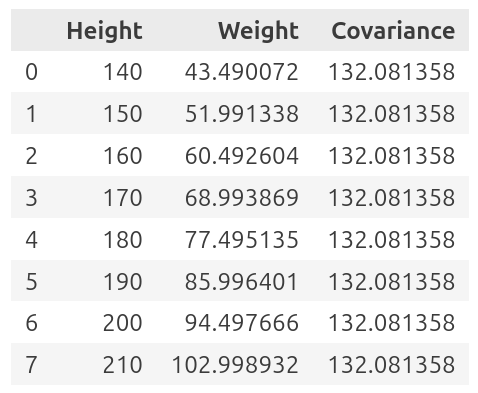
\includegraphics[width=0.7\textwidth]{images/predictions.png}
        \end{center}
        \end{column}
        \begin{column}{0.5\textwidth}  
        \begin{figure}
            \centering
            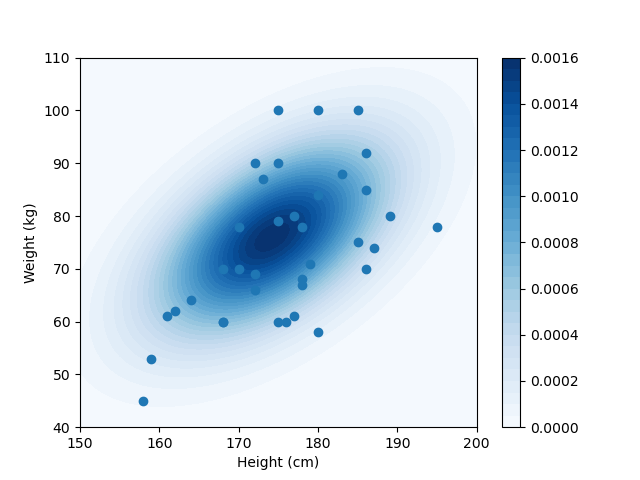
\includegraphics[width=0.7\textwidth]{images/gaussian.png}
            \caption{Estimated PDF and given data}
            \end{figure}
        \end{column}
    \end{columns}
\end{frame}

\begin{frame}
    \frametitle{Task 2.1.3 :: Pondering}

    \begin{itemize}
        \item[+] Results seem plausible -- can mostly judge are around mean though
        \item[-] Fixed variance doesnt match expectations
        \begin{itemize}
            \item maybe taller people $\rightarrow$ more variance?
            \item there are more average sized people $\rightarrow$ maybe more variance? 
        \end{itemize}
        \item[-] Cube-Square-Law / BMI suggests a non-linear / quadratic relationship?
        \item    Plausibility? Test-Set and more 'human-readable' metrics!
    \end{itemize}
\end{frame}

\section{2.2}
\begin{frame}
    \frametitle{Task 2.2.1 :: Loading}
    \begin{columns}
    \begin{column}{0.6\textwidth}
        \inputminted[bgcolor=LightGray,fontsize=\small]{python}{code/myspace-pre.py}
    \end{column}
    \begin{column}{0.4\textwidth}
        \begin{figure}
            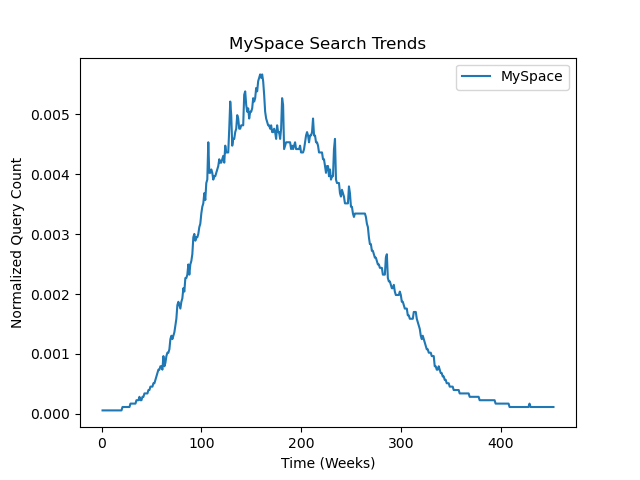
\includegraphics[width=\textwidth]{images/myspace.png}
        \end{figure}
    \end{column}
    \end{columns}
\end{frame}

\begin{frame}
    \frametitle{Task 2.2.1 :: ManuDiff Newton}
\end{frame}

\section{2.3}
\begin{frame}
    \frametitle{Task 2.3 :: Scipy CurveFit}
    \inputminted[bgcolor=LightGray,fontsize=\small]{python}{code/curve-fit.py}

    \begin{columns}
        \begin{column}{0.7\textwidth}
            \begin{itemize}
                \item mostly works just like that
                \item could have also scaled the data (see 2.5) \\
                        instead of adding the amplitude parameter
            \end{itemize}
        \end{column}
    
        \begin{column}{0.3\textwidth}
            \begin{figure}
                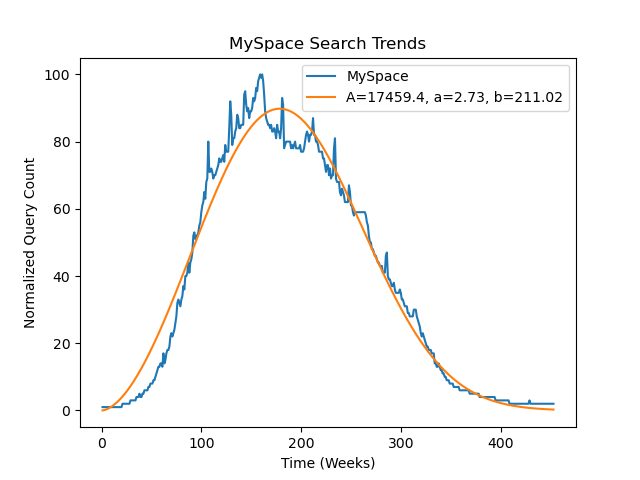
\includegraphics[width=\textwidth]{images/scicurvefit.png}
            \end{figure}
        \end{column}
        \end{columns}
\end{frame}

\section{2.4}
\begin{frame}
    \frametitle{Task 2.4}
\end{frame}

\section{2.5}
\begin{frame}
    \frametitle{Task 2.5 :: Scipy Minimize}
    \inputminted[bgcolor=LightGray,fontsize=\small]{python}{code/minimize-kl.py}

    \begin{columns}
    \begin{column}{0.7\textwidth}
        \begin{itemize}
            \item Bounds are important, but also not: $[-\infty, \infty]$ works, too
            \item Feels odd anyway, because a gradient method optimizing \\ 
                    1 $\rightarrow$ 2.8 shouldn't come near 0 anyway
            \item[$\Rightarrow$] Adding bounds just change the algorithm underneath
            \item Without bounds 'BFGS' is choosen and doesnt quite work
            \item 'L-BFGS-B' or 'SLSQP' without bounds works equally well
        \end{itemize}
    \end{column}

    \begin{column}{0.3\textwidth}
        \begin{figure}
            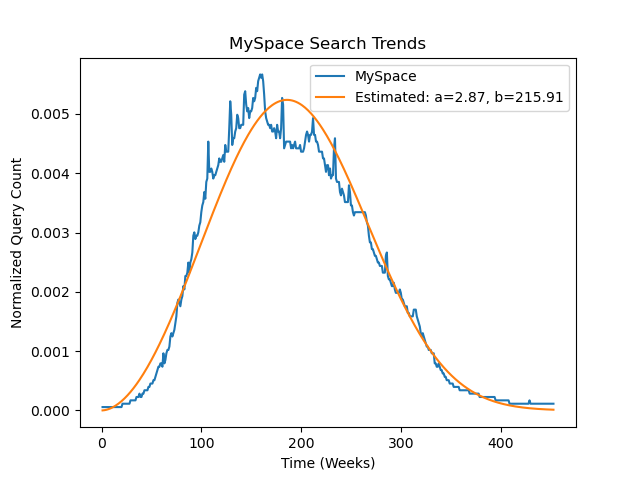
\includegraphics[width=\textwidth]{images/sciminimize.png}
        \end{figure}
    \end{column}
    \end{columns}

\end{frame}

\end{document}
